\section{Introduction}

\textcolor{black}{Combinatorial optimization problems on graphs arise in many application domains, including social networks, transportation, telecommunications, and scheduling, and are typically NP-hard. For instance, in facility location problems such as opening retail outlets under a budget constraint, many candidate sites are unpromising due to high costs, low demand, or redundancy with nearby locations. In fact, among the 21 NP-complete problems introduced by Karp \citep{karp2009reducibility}, 10 are decision versions of graph optimization problems, while most of the remaining problems, such as set covering, can be naturally formulated on graphs.} Several heuristics have been developed to obtain near-optimal solutions, but they do not typically scale well with problem size. Pruning the ground set to a smaller pool of promising candidates enables heuristics and exact methods to scale more efficiently without sacrificing solution quality.




\begin{figure*}[t]
    \centering
    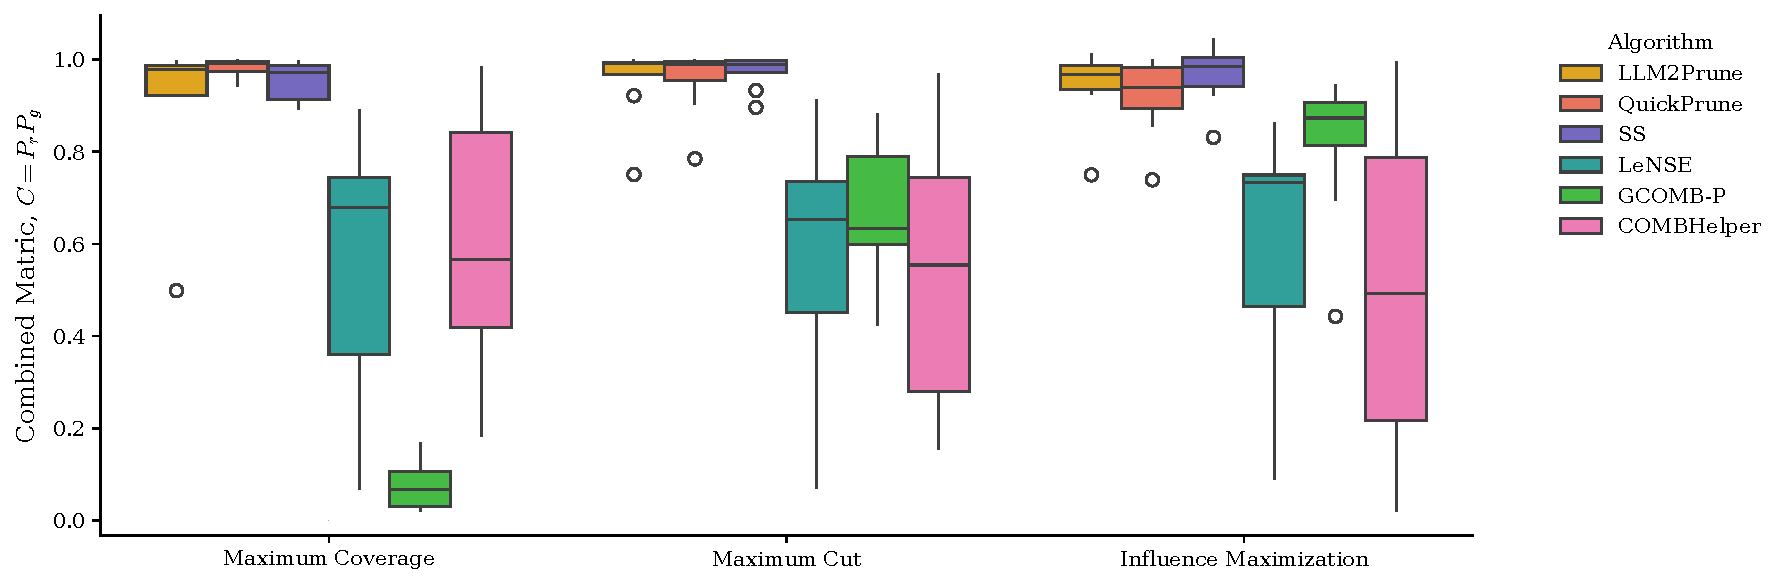
\includegraphics[width=\linewidth]{figures/algorithm_comparison_boxplot.pdf}
    % \caption{Caption}
   \caption{Comparison of pruning algorithms across three CO problems. The boxplots report the combined metric $C = P_r P_g$ (defined below), which balances solution quality and ground set reduction. \llm \textcolor{black}{(ours)} is competitive with classical approaches (\qp, SS) and outperforms learning-based approaches (GCOMB, \lense, \comb) by a large margin, without relying on domain knowledge.}


    \label{fig:boxplot}
\end{figure*}

In this work, we study the problem of identifying a smaller subset of the ground set for \textcolor{black}{graph optimization problems}, where the goal is to maximize or minimize an objective function over a large discrete configuration space subject to constraints. Formally, we have the following problem definition \textcolor{black}{for the general CO problem}.

 % The goal is to find a feasible solution \( x \in S \) that minimizes or maximizes \( f(x) \) subject to all constraints in \( \Omega \). Since most CO problems are NP-hard, no polynomial-time algorithms are known to solve them in the general case. So we have the following problem definition

\textbf{Problem Definition (Pruning).} A CO problem can be expressed as the tuple \( (S, \Omega, f) \), where \( S \) denotes the search space over discrete decision variables, \( \Omega \) represents the set of constraints that define feasibility, and \( f: S \to \mathbb{R} \) is the objective function to be optimized.
Given a CO problem with ground set \(\mathcal{U}\) and an exact solver \(\mathcal{OPT}\), the optimal solution is  
\[
X^\star = \mathcal{OPT}(\mathcal{U}) = \arg\max_{X \subseteq \mathcal{U}, \; X \text{ satisfies } \Omega} f(X)
\]  
The pruning problem seeks to construct a much smaller ground set \(\mathcal{U}'\) with \(|\mathcal{U}'| \ll |\mathcal{U}|\), such that solving the reduced instance yields nearly the same objective value:  
\[
\frac{f(\mathcal{OPT}(\mathcal{U}'))}{f(\mathcal{OPT}(\mathcal{U}))} = 1 - \epsilon
\]  
for a small approximation factor \(\epsilon \geq 0\).  

% Existing pruning approaches face several limitations: (i) limited scalability \citep{zhou2017scaling,pmlr-v258-nath25a};  (ii) reliance on handcrafted, problem-specific features requiring domain expertise \citep{ireland2022lense,tian2024combhelper}; (iii) lack of problem-agnostic pipelines or weak performance on general graph optimization tasks \citep{lauri2019fine,lauri2023learning,manchanda2020gcomb}; and (iv) poor adaptability to constraints, a limitation shared by all these methods. 
\textcolor{black}{Existing pruning approaches are limited by scalability issues \citep{zhou2017scaling,pmlr-v258-nath25a}, reliance on handcrafted problem-specific features \citep{ireland2022lense,tian2024combhelper}, lack of problem-agnostic pipelines or weak performance on general graph optimization problems \citep{lauri2019fine,lauri2023learning,manchanda2020gcomb}, and poor adaptability to constraints.} Thus, in this work, we are motivated by the following question:
\begin{center}
    \textcolor{black}{\textit{Is it possible to design a scalable pruning framework that avoids handcrafted features, delivers strong performance across general CO problems over graphs, and adapts easily to constraints?}}
\end{center}

\textcolor{black}{To address these limitations, we propose \llm, a framework that replaces prior supervised methods relying on problem-specific, hand-crafted features that limit generality across \textcolor{black}{graph optimization problems} and constraints} In addition, it overcomes classical methods that use sequential pruning, which struggle with scalability. Our approach uses LLMs to automatically generate features for a downstream classifier, which is then applied to prune the ground set of a \textcolor{black}{graph optimization} problem. Given a problem definition, we employ an LLM-guided beam search over the feature space, directed by both performance evaluation and feature importance scores. These signals act as surrogate gradients, steering the search toward high-quality features that improve the performance of the downstream classifier. In contrast, prior works that employ LLMs for feature generation either rely on manually specified rules, derive new features only from existing ones, or use simple feedback loops that allow error propagation and lack feature-importance guidance. By comparison, our approach generates features in a guided search framework that balances exploration with structured signals, making it robust to noisy feedback and enabling consistent feature discovery.


% To this end, we propose leveraging the reasoning capabilities of 



% Contrast with supervised pruning. Prior supervised methods rely on problem-specific, hand-crafted features and iterative, sequential pruning, which limits generality and scalability. LLM2Prune replaces manual feature design with LLM-generated, task-aware features, uses semi-supervised training to mitigate label noise from weak labels, and performs single-shot universe pruning guided by feature-importance—yielding faster pipelines that generalize across CO tasks while preserving quality.

\textbf{Contributions.}  
Our work makes the following contributions:  



\begin{itemize}
    % \item We propose \llm, a framework that leverages the reasoning capabilities of LLMs to automatically generate features for a lightweight classifier that prunes the search space of CO problems, avoiding hand-crafted, problem-specific engineering.  
    \item \textcolor{black}{We propose \llm, a framework that leverages the reasoning capabilities of LLMs to automatically generate features for a lightweight classifier that prunes the search space of  \textcolor{black}{CO problems over graphs}. Unlike prior approaches, it avoids hand-crafted, problem-specific engineering and can easily adapt to constraints.}
    \item We introduce an LLM-guided beam search strategy for feature generation that incorporates feature-importance score and performance evaluation. This approach overcomes the limitations of a simple feedback loop by maintaining diversity and stability in feature exploration.
    % Feature-importance vectors, together with performance evaluation, serve as surrogate gradients to guide effective feature discovery.
    \item \textcolor{black}{We evaluate \llm on diverse graph optimization problems under both size and knapsack constraints. Under size constraints, \llm achieves solution quality comparable to classical methods while enabling substantially faster pruning. It consistently outperforms state-of-the-art learning-based pruning approaches in solution quality and runtime. The ability of \llm to adapt naturally to additional constraints is demonstrated under knapsack constraints, where it achieves superior performance compared to existing methods.}
    % and find that it delivers comparable or better solution quality than state-of-the-art pruning algorithms (Figure \ref{fig:boxplot}), while achieving faster pruning and producing a much smaller ground set.  
\end{itemize}

\textbf{Organization.} The rest of this paper is organized as follows. In Section \ref{sec:related_work}, we describe the relationship between our contribution and existing work. In Section \ref{sec:method}, we present our algorithm, \llm, and conduct an empirical evaluation, comparing it to existing learned and classical heuristics for the pruning problem, followed by a discussion of limitations and future directions. Finally, in Section \ref{section:conclusion}, we conclude the paper.

    % \item We propose \textbf{LLM2Prune}, a framework that leverages the reasoning capabilities of LLMs to automatically generate features for a lightweight classifier to prune in a single step, avoiding hand-crafted, problem-specific engineering.  
    % \item Our approach introduces an LLM-guided beam search strategy and exploit semi-supervised learning to reduce label noise. The performance evaluation and feature importance signals act as surrogate gradients for effective feature discovery in feature search space. The beam search makes the framework robust to noisy feedback from LLMs.
    % \item We conduct extensive experiments on multiple CO tasks under size and knapsack constraints and demonstrate that LLM2Prune
    % outperforms learning baselines and is order-of-magnitude faster than classical methods at comparable quality.
    % achieves strong performance while significantly reducing the ground set size, outperforming both problem-specific and problem-agnostic baselines.  









 

    
